\section{Ideal flow: planar 2-dimensional potential flow around cylinder (26-36)}

\begin{framed}
For further details see section 4.3, 4.9 and 7.1-3 in the KCD book
\end{framed}

\begin{shaded}
I skipped the summary of NS equation on page 26 of hand written notes. Maybe there should be an introductory paragraph here with references to equations from previous sections.
\end{shaded}

\begin{figure}[!h]
    \centering
    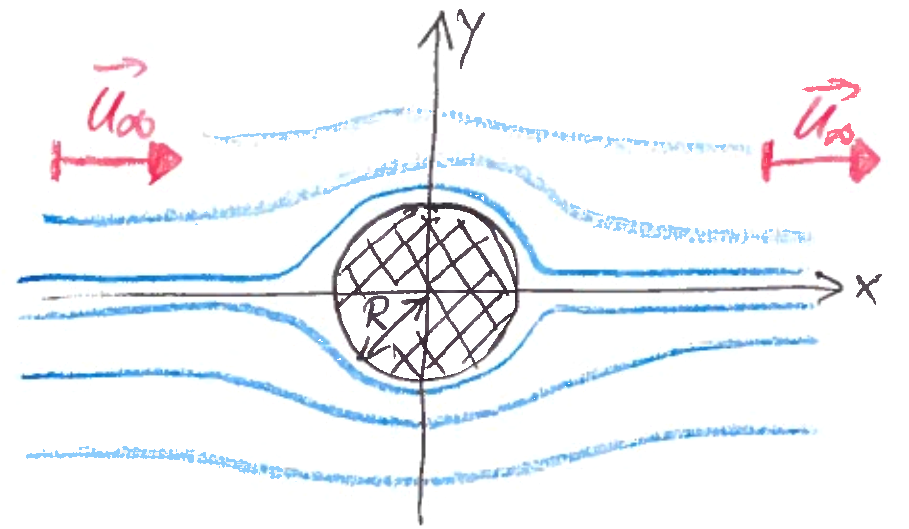
\includegraphics[width=.5\textwidth]{week3/planar-flow}
    \caption{}
    \label{fig:planar-flow}
\end{figure}

Questions to \fref{fig:planar-flow}: 1) $\vec{u} = \vec{u}(x,y,z)$?, 2) pathlines (streamlines)?

\begin{equation}
\vec{\nabla}\times\vec{u} = 0 \Rightarrow \vec{u}(\vec{r}) = \vec{\nabla}\phi(\vec{r})
\end{equation}
where $\phi(\vec{r})$ is a velocity potential.

\begin{align}
\vec{\nabla}\times\vec{u} &= 0\\
\leadsto
\vec{\nabla}\cdot\vec{\nabla}\phi(\vec{r}) &= \left(\ppdiff{}{x}+\ppdiff{}{y}+\ppdiff{}{z}\right)\phi(x,y)\\
&= \left(\ppdiff{}{x}+\ppdiff{}{y}\right)\phi(x,y) = 0
\end{align}
This second order differential equation is the Laplace equation.

Question: How does the cylinder (obstacle) enter in solving the Laplace equation?

Two boundary conditions.

1:
\begin{align}
\vec{u}(|\vec{r}|\rightarrow\infty) &= \vec{u}_\infty = u_\infty\vec{e}_x \\
\leadsto
\phi(|\vec{r}|\rightarrow\infty) &= u_\infty x + \mathrm{constant}
\end{align}

2:
\begin{equation}
0=u_\mathrm{surface}\cdot \vec{n} = \vec{\nabla}\phi\biggm\vert_\mathrm{surface}\cdot\vec{n}
\end{equation}

The fluid particle does not flow into the surface; only tangential component.

\begin{figure}[!h]
    \centering
    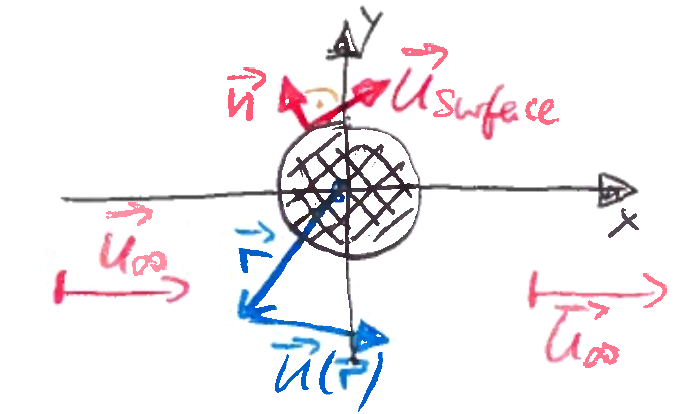
\includegraphics[width=.5\textwidth]{week3/planar-flow2}
    \caption{}
    \label{fig:planar-flow2}
\end{figure}

For the flow around the cylinder the solution of the Laplace equation with the two boundary conditions "falls from the sky" (for the moment):
\begin{equation}
\phi(x,y)=u_\infty\times\left(1+\frac{R^2}{x^2+y^2}\right)
\end{equation}

\begin{shaded}
I skipped the last part of page 28 here
\end{shaded}

Velocity field:
\begin{equation}
\vec{u} = \begin{pmatrix}
u_x\\u_y
\end{pmatrix}  = 
\vec{\nabla}\phi(x,y) = \begin{pmatrix}
\pdiff{\phi}{x} \\
\pdiff{\phi}{y}
\end{pmatrix}
\end{equation}

\begin{align}
\begin{split}\label{eq:uxuy1}
u_x &= u_\infty\left(1+\frac{R^2(y^2-x^2)}{(x^2+y^2)^2}\right)\\
u_y &= -u_\infty \frac{2xyR^2}{(x^2+y^2)^2}
\end{split}
\end{align}

\begin{figure}[!h]
    \centering
    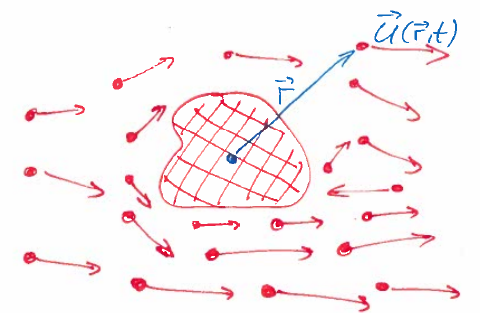
\includegraphics[width=.7\textwidth]{week3/velocity-field}
    \caption{}
    \label{fig:velocity-field}
\end{figure}

examples:
\begin{align}
\vec{u}\biggm\vert_{x\rightarrow\pm\infty} &= u_\infty\vec{e}_x = \vec{u}\biggm\vert_{y\rightarrow\pm\infty}\\
\vec{u}\biggm\vert_{\small\vec{r}=\begin{pmatrix} 0 \\ R
\end{pmatrix}} &= 2u_\infty\vec{e}_x \\
\vec{u}\biggm\vert_{\small\vec{r}=\begin{pmatrix} R \\ 0
\end{pmatrix}} &= 0 = \vec{u}\biggm\vert_{\small\vec{r}=\begin{pmatrix} -R \\ 0
\end{pmatrix}}
\end{align}


\newpage
\subsection{Pathline around a cylinder}

\begin{figure}[!h]
    \centering
    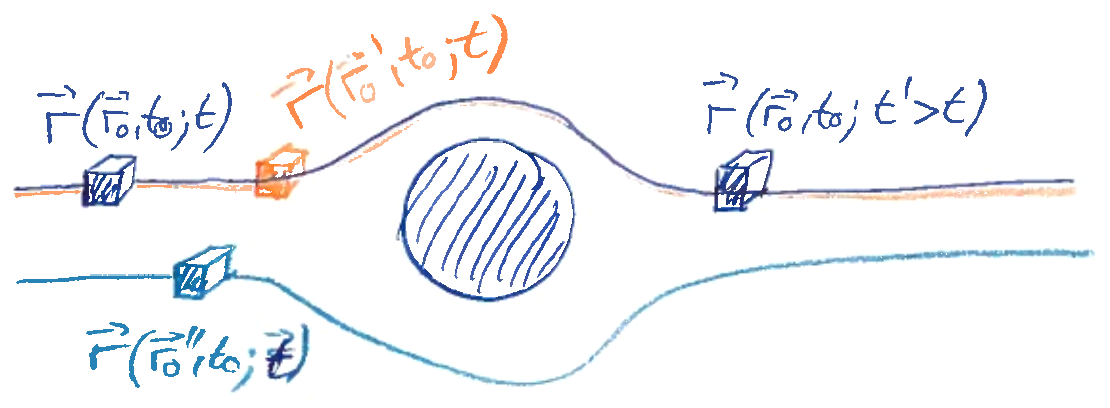
\includegraphics[width=.7\textwidth]{week3/pathline-cylinder}\\
    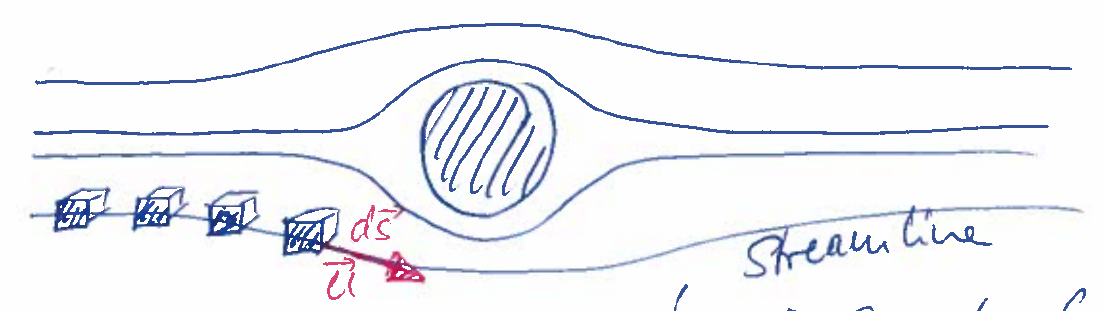
\includegraphics[width=.7\textwidth]{week3/pathline-cylinder2}
    \caption{}
    \label{fig:pathline-cylinder}
\end{figure}

Top part of \fref{fig:pathline-cylinder} shows the Lagrangian picture: follows particle through all times. the bottom part shows the Eulerian picture, which is a snapshot of all fluid particles at one particular time.

Connection between Lagrangian and Eulerian picture:
\begin{equation}
\diff{\vec{r}}{t} = \vec{u}(\vec{r},t)
\end{equation}

For stationary flows
\begin{equation}
\vec{u}(\vec{r},t)=\vec{u}(\vec{r}) \Rightarrow \mathrm{pathline} = \mathrm{streamline}
\end{equation}

Given the snapshots $\vec{u}(\vec{r},t)$, we can calculate the pathlines.

Given the pathlines, we can construct the snapshots.

This sounds like the "chicken and egg" problem.

\bigskip
Question: How to calculate the streamlines?

First approach:
Definition of streamline:
\begin{equation}
d\vec{s}\parallel\vec{u},
\end{equation}
where $ds$ is a line element of a streamline.
\begin{align}
0=d\vec{s}\times\vec{u} &=
\begin{vmatrix}
0 & 0 & \vec{e}_z \\
dx & dy & 0 \\
u_x & u_y & 0
\end{vmatrix} =
(u_ydx-u_xdy)\vec{e}_z\\
\leadsto
\diff{y}{x} &= \frac{u_y}{u_x} = -\frac{2xyR^2}{(x^2+y^2)^2+R^2(y^2-x^2)}
\end{align}

Second approach: introduce the streamfunction $\psi(x,y)$.

Incompressibility gives us:
\begin{equation}
 \vec{\nabla}\cdot\vec{u} = \pdiff{u_x}{x}+\pdiff{u_y}{y}=0
\end{equation}
which leads to
\begin{equation}
 u_x = \pdiff{\psi}{y}, \quad u_y = -\pdiff{\psi}{x} \label{eq:uxuy2}
\end{equation}

\begin{align}
d\vec{s}\times\vec{u} &= (u_ydx-u_xdy)\vec{e}_x \\
&= \left(-\pdiff{\psi}{x}dx-\pdiff{\psi}{y}dy\right)\vec{e}_z\\
&= -d\psi \vec{e}_z \require 0
\end{align}
The streamfunction is constant along a streamline. This represents an \emph{isopotentialline} of the streamfunction and describes a streamline.

From the defining functions of the streamfunction in \eqref{eq:uxuy2} and the $u_x$, $u_y$ solution for the ideal flow around a cylinder in \eqref{eq:uxuy1}, we can determine $\psi$ by partial integration
\begin{align}
\psi(x,y) &= v_\infty y\left(1-\frac{R"2}{x^2+y^2}\right)\\
&= v_\infty \sin\psi\left(r-\frac{R^2}{r}\right)
\end{align}

\begin{framed}
\textbf{Remark:} relationship between velocity potential and streamfunction $\phi=\mathrm{constant}$, $\psi=\mathrm{constant}$ represent and orthogonal set of curves, because
\begin{equation}
\left(\vec{\nabla}\phi\right)\cdot\left(\vec{\nabla}\psi\right) = 
\begin{pmatrix}
\pdiff{\phi}{x} \\ \pdiff{\phi}{y}
\end{pmatrix} \cdot
\begin{pmatrix}
\pdiff{\psi}{x} \\ \pdiff{\psi}{y}
\end{pmatrix} = 
\begin{pmatrix}
u_x \\ u_y
\end{pmatrix}\cdot
\begin{pmatrix}
-u_y \\ u_x
\end{pmatrix} = 0
\end{equation}
\end{framed}

\begin{shaded}
I left out page 32a-32d here.
\end{shaded}

Two dimensional potential flow around an infinitely long cylinder 

Because of cylinder symmetry we can transform from  to cylindrical coordinates
\begin{align}
x &= r\cos\phi\\
y &= r\sin\phi
\end{align}

\begin{equation}
\Phi(x,y) \rightarrow \Phi(r,\phi)
\end{equation}

\begin{align}
\Delta\Phi(x,y) &= \left(\ppdiff{}{x}+\ppdiff{}{y}\right)\Phi(x,y) \\
&= \left[\frac{1}{r}\pdiff{}{r}\left(r\pdiff{}{r}\right) + \frac{1}{r^2}\pdiff{}{\phi}\right]\Phi(r,\phi)\\
&= 0\\
\leadsto
r\pdiff{}{r}\left(\pdiff{\Phi}{r}\right) &= -\ppdiff{\Phi}{\phi}
\end{align}

\begin{shaded}
I left out page 33a-33b here.
\end{shaded}

Ansatz: factorization
\begin{equation}
\Phi(r,\phi) = f(r)g(\phi)
\end{equation}

\begin{align}
\frac{1}{f\cdot g} r\pdiff{}{r}\left(r\pdiff{(f(r)g(\phi))}{r}\right) &= -\frac{1}{f\cdot g}\ppdiff{(f(r)g(\phi))}{\phi} \\
\leadsto
\frac{1}{f(r)}r\pdiff{}{r}\left(r\pdiff{f(r)}{r}\right) &= -\frac{1}{g(\phi)}\ppdiff{g(\phi)}{\phi} \require m^2
\end{align}

Left part depends only on $r$, middle part depends only on $\phi$, and right part is a constant, which does neither depend on $r$ nor $\phi$.

\begin{align}
\ppdiff{g(\phi)}{\phi} &= -m^2g(\phi)\\
\leadsto
g(\phi) = e^{im\phi} &=  \cos m\phi + i\sin m\phi
\end{align}

requirement:
\begin{align}
g(\phi) &= g(\phi+2\pi)\\
\leadsto
e^{im\phi} &= e^{im(\phi+2m)}\\
\leadsto
e^{2\pi im} &= 1
\end{align}

\begin{equation}
r\pdiff{}{r}\left(r\pdiff{}{r}f(r)\right) = m^2f(r)
\end{equation}

polynomial ansatz:
\begin{equation}
f(r) = r^\alpha
\end{equation}

\begin{align}
r\pdiff{}{r}\left(r\alpha r^{\alpha-1}\right) &= \alpha^2 r^\alpha \require m^2 r^\alpha\\
leadsto
\alpha &= \pm m
\end{align}

\begin{equation}
\Phi(r,\phi) = f(r)g(\phi) = r^{\pm m}e^{im\phi}
\end{equation}

Since the Laplace equation is linear in $\Phi$, the most general solution for $\Phi$ is a linear superposition of all possible solutions:
\begin{align}
\Phi(r\phi) &= \sum_{m=-\infty}^\infty \left(a_m r^m + b_m r^{-m}\right) e^{im\phi} \\
&= \sum_{m=1}^{\infty} \left[ \left(a_m r^m + b_m r^{-m}\right)e^{im\phi} + \left(c_m r^m + d_m rÅ {-m}\right) e^{-im\phi}\right]
\end{align}

Remark:
\begin{align}
\Phi_{m=0} &= a_0+b_0 = \mathrm{constant} \\
\leadsto
\vec{u}_{m=0} &= \vec{\nabla}\Phi_{m=0}=0
\end{align}

Determination of amplitudes $a_m$, $b_m$, $c_m$, and $d_m$ via boundary conditions:

\begin{equation}
\Phi(r\rightarrow\infty, \phi) = u_\infty x = u_\infty r\cos\phi
\end{equation}

\begin{equation}
\vec{u}\cdot \vec{e}_r |_{r=R} = \vec{\nabla}\Phi\cdot\vec{e}_r|_{r=R} = \pdiff{\Phi}{r}\biggm\vert_{r=R}=0
\end{equation}

\begin{shaded}
I left out the derivations on page 36
\end{shaded}

\begin{equation}
\Phi(r,\phi) = u_\infty r \cos \phi \left(1+\frac{R^2}{r^2}\right) = u_\infty x \left(1+\frac{R^2}{x^2+y^2}\right) = \Phi(x,y)
\end{equation}



\section{Ideal potential flows (continued) (37-44)}

\begin{framed}
\textbf{Opening remark:} 2-dimensional potential flow solutions will often look like
\begin{equation}
\Phi(x,y) = u_\infty x + f(x,y).
\end{equation}
Any function $f(x,y)$, which fulfills
\begin{equation}
\ppdiff{f}{x}+\ppdiff{f}{y}=0 \qquad \mathrm{and}\qquad f(|x|,|y|\rightarrow\infty) = 0,
\end{equation}
describes a flow around some obstacle.
\end{framed}


\textbf{Play 1:}
\begin{equation}
\Phi(x,y)=\frac{m}{2\pi} \ln \sqrt{x^2+y^2}
\end{equation}
represents the radial flow resulting from a source with strength $m$. See \fref{fig:radial-streamlines}.
\begin{figure}[!h]
    \centering
    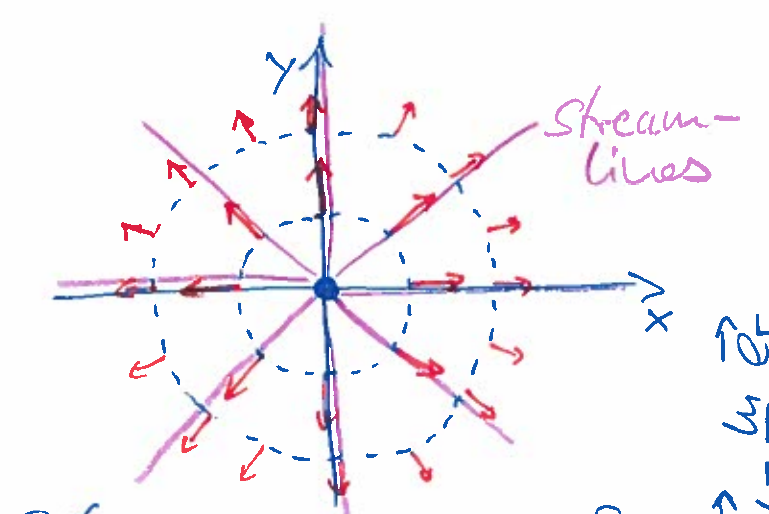
\includegraphics[width=.5\textwidth]{week3/radial-streamlines}\\
    \caption{}
    \label{fig:radial-streamlines}
\end{figure}

\textbf{Play 2:} method of images. Source flow in front of a wall. See \fref{fig:mirror-source}.

Boundary condition: no flow through the wall; only tangential component.
\begin{equation}
\phi(x,y) = \frac{m}{2\pi}\ln\sqrt{(x+a)^2+y^2} + \frac{m}{2\pi}\ln\sqrt{(x-a)^2+y^2}
\end{equation}
\begin{figure}[!h]
    \centering
    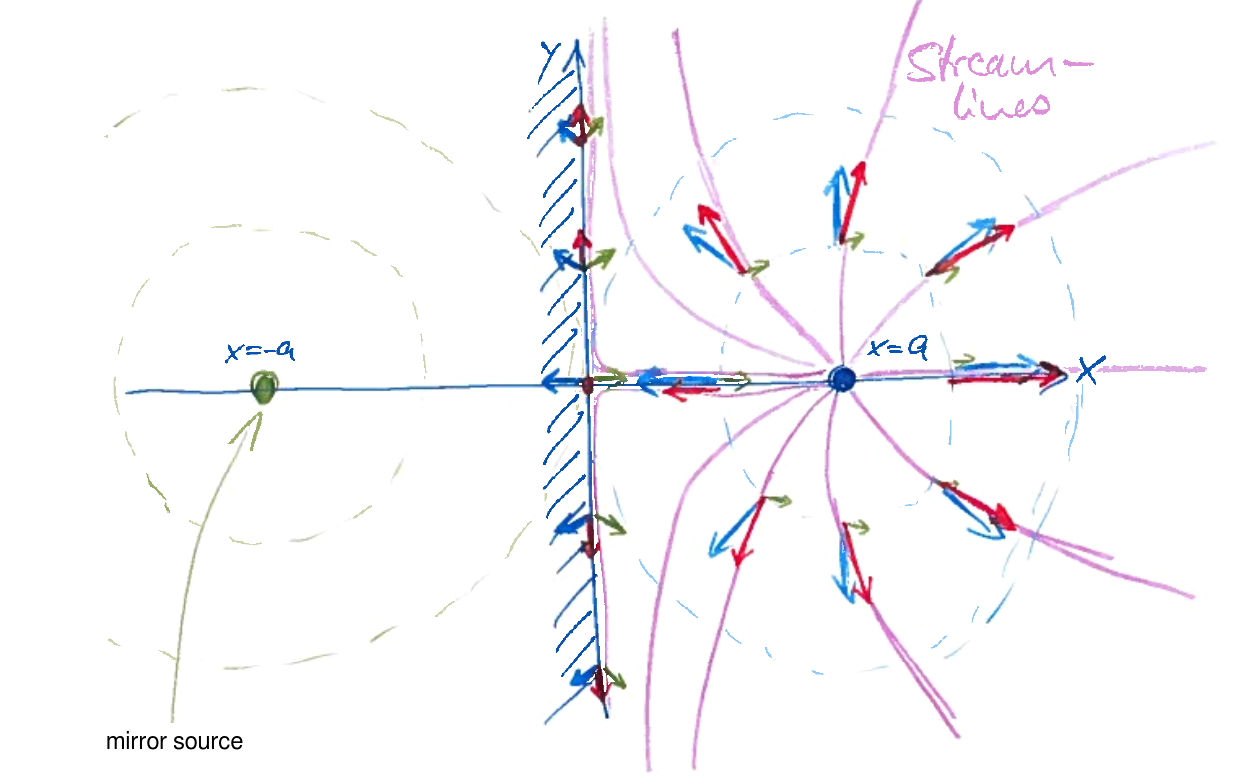
\includegraphics[width=.6\textwidth]{week3/mirror-source}\\
    \caption{}
    \label{fig:mirror-source}
\end{figure}

\textbf{Play 3:} flow past a 2-dimensional half-body. See \fref{fig:half-body}.
\begin{align}
\Phi &= u_\infty x + \frac{m}{2\pi}\ln\sqrt{x^2+y^2}\\
\leadsto
\ppdiff{\Phi}{x}+\ppdiff{\Phi}{y} &= 0
\end{align}
\begin{align}
u_x(x,y) &= u_\infty + \frac{m}{2\pi}\frac{x}{x^2+y^2}\\
u_y(x,y) &= u_\infty + \frac{m}{2\pi}\frac{y}{x^2+y^2}
\end{align}

Engineering flow interpretations:
\begin{enumerate}
\item An example of the beginning of the half-body is the leading edge of an airfoil
\item pedestrian on a bridge looking down: front part of a bridge pier
\item flow over a cliff
\end{enumerate}

\begin{figure}[!h]
    \centering
    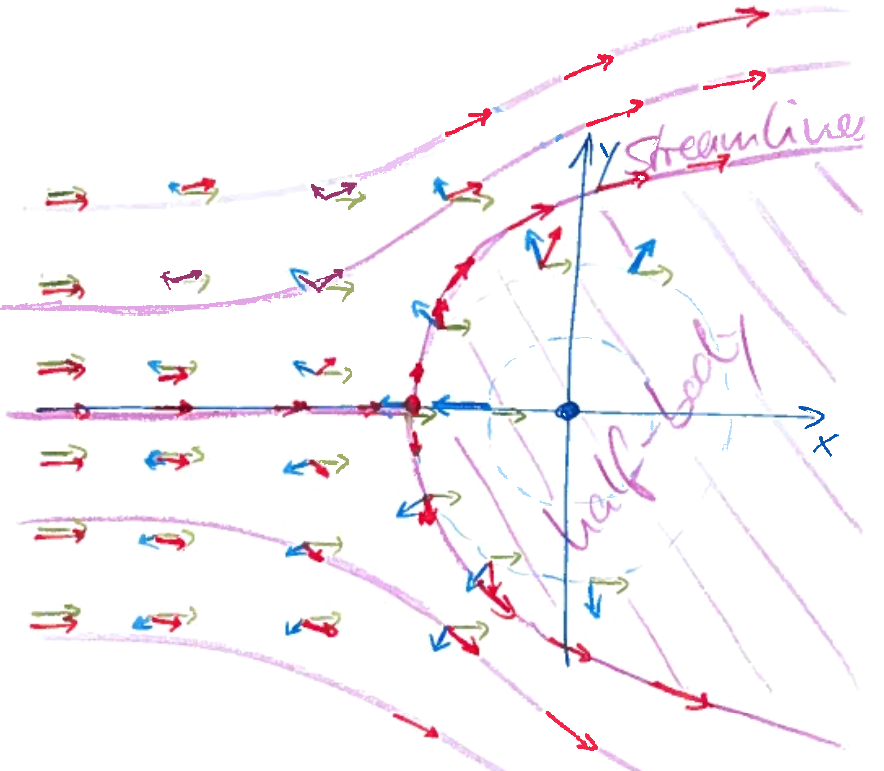
\includegraphics[width=.6\textwidth]{week3/half-body}\\
    \caption{}
    \label{fig:half-body}
\end{figure}

\textbf{Play 4:} numerial solutions (KCD section 6: Computational Fluid Dynamics)

\textbf{Play 5:} "beauty of mathematics". Conformal mappings.
Complex potential
\begin{equation}
w(z) = \phi(x,y)+i\psi(x,y)
\end{equation}
where $z=x+iy$.

Velocity:
\begin{align}
\diff{w(z)}{z} &= \diff{w(z)}{z}\biggm\vert_{dz=dx} = \pdiff{\phi}{x}+i\pdiff{\psi}{x} = u_x-iu_y \\
&= \diff{w(z)}{z}\biggm\vert_{dz=idy} = \pdiff{\phi}{y}+i\pdiff{\psi}{y} = \pdiff{\psi}{y}-i\pdiff{\phi}{y} = u_x-iu_y
\end{align}

Differentiable example 1:
\begin{equation}
w(z)=u_\infty z = u_\infty(x+iy) = u_\infty x + iu_\infty y
\end{equation}
describes the constant flow $\vec{u}=u_\infty \vec{e}_x$.

Differentiable example 2:
\begin{align}
w(z) &= \frac{m}{2\pi}\ln z = \frac{m}{2\pi} \ln(x+iy)\\
&= \frac{m}{2\pi}\ln(re^{i\theta}\\
&= \frac{m}{2\pi}\ln r +\frac{m}{2\pi}\ln e^{i\theta}\\
&= \frac{m}{2\pi}\ln\sqrt{x^2+y^2} + i\frac{m}{2\pi}\theta
\end{align}
The two terms in the last line is the velocity field and stream function of a radial source flow (see "play 1").

Differentiable example 3:
\begin{align}
w(z) &= \frac{A}{2}z^2 = \frac{A}{2}(x+iy)^2\\
&= \frac{A}{2}(x^2-y^2)+iAxy
\end{align}

Differentiable example 4:
\begin{align}
w(z) &= \phi(x,y) +i\psi(x,y) = u_\infty x\left(1+\frac{R^2}{x^2+y^2}\right) + iu_\infty y \left(1-\frac{R^2}{x^2+y^2}\right) \\
& =u_\infty(x+iy) + u_\infty R^2\frac{x-iy}{x^2+y^2} \\
&= u_\infty(x+iy)+\frac{u_\infty R^2}{x+iy}\\
&= u_\infty\left(z+\frac{R^2}{z}\right)
\end{align}

flow around cylinder with radius $R$:
\begin{equation}
w(z)=u_\infty\left(z+\frac{R^2}{z}\right)
\end{equation}
change of variable:
\begin{equation}
z)z(\tilde{z})
\end{equation}
Example:
\begin{align}
\tilde{z} &= (z+z_0)+\frac{1}{z+z_0}\\
\leadsto
w_\mathrm{new\ obstacle}(\tilde{z}) &= w_\mathrm{cylinder}(z(\tilde{z}))
\end{align}

\begin{shaded}
Should we include the figure on the left half of page 43 here?
\end{shaded}


\begin{framed}
\textbf{Remark:} other applications of conformal mappings

\textbf{Electrostatics}
\begin{equation}
\Delta\phi = \vec{\nabla}\cdot\vec{\nabla\phi=0}
\end{equation}

\textbf{Heat flux}
\begin{equation}
\pdiff{T(x,y)}{t}=\kappa\vec{\nabla}\cdot\vec{\nabla}T(x,y) \Rightarrow \Delta T(x,y) = 0
\end{equation}
\end{framed}
